\documentclass[11pt,a4paper]{article}
\usepackage[T1]{fontenc}
\usepackage{newtxtext,newtxmath}
\usepackage[margin=24mm,headheight=15pt]{geometry}
\usepackage{graphicx}
\usepackage[font=small,labelfont=bf]{caption}
\usepackage{microtype}
\usepackage{fancyhdr}
\usepackage{parskip}
\usepackage{titlesec}
\usepackage{natbib}
\usepackage[hidelinks]{hyperref}

\renewcommand*{\figureautorefname}{Figure}
\renewcommand*{\tableautorefname}{Table}
\renewcommand*{\equationautorefname}{Equation}
\hypersetup{
  linktoc=all,
  pdfstartview=Fit,
  pdftitle={Patch-Based Diffusion Models for Solving Inverse Problems in Computed Tomography Imaging -- Executive Summary},
  pdfauthor={Thomas Hartigan},
  pdfsubject={Data Intensive Science},
  pdfkeywords={computed tomography, diffusion models, PaDIS, reproducibility, inverse problems}
}

\let\filledcite\cite
\renewcommand{\cite}[1]{%
  \if\relax\detokenize{#1}\relax
    \unskip
  \else
    \filledcite{#1}%
  \fi
}

\pagestyle{fancy}
\fancyhf{}
\lhead{\small Executive Summary}
\rhead{\small Thomas Hartigan}
\cfoot{\small\thepage}
\renewcommand{\headrulewidth}{0.4pt}
\titleformat{\section}{\large\bfseries}{}{0pt}{}
\titlespacing*{\section}{0pt}{1.1em}{0.35em}

\begin{document}

\begin{center}

\includegraphics[width=14mm]{Figs/University_Crest.pdf}\\[0.35em]
{\LARGE\bfseries Patch-Based Diffusion Models for Solving\\[0.15em]Inverse Problems in Computed Tomography Imaging}\\[0.45em]
{\large Executive Summary}\\[0.3em]
{\normalsize Thomas Hartigan \enspace $\vert$ \enspace MPhil in Data Intensive Science}\\[0.45em]
\rule{\textwidth}{0.6pt}
\end{center}

\section{Purpose and Motivation}

Computed tomography (CT) reconstructs anatomy from X-ray measurements \cite{}. Fewer projection angles can reduce acquisition time and radiation exposure, but leave reconstruction underdetermined because many images explain sparse measurements. Classical methods therefore produce streaking or blur without a prior for plausible anatomy.

Diffusion models provide expressive learned priors, although whole-image models can require extensive data, training and GPU memory \cite{}. Hu et al. proposed the Patch Diffusion Inverse Solver (PaDIS) \cite{}. PaDIS trains on position-labelled patches and changes their partitions during reconstruction, combining local scores into a whole-image update intended to remove seams. In the original PaDIS paper, Hu et al. reported that PaDIS consistently outperformed a comparable whole-image diffusion model on sparse-view CT.

This work tested whether that result could be reproduced on a public dataset with a specified fan-beam geometry, and which choices drive performance. Independent testing matters because hidden implementation choices hinder validation, making this a reproduction and extension rather than a numerical rerun.

\section{Approach}

Training, tuning and evaluation were reimplemented within LION \cite{} rather than treating the released code as executable ground truth. Patient-separated LIDC-IDRI slices provided the data \cite{}. The default subset contained at most four slices per patient, while an ablation used every processed slice. A fully specified two-dimensional fan-beam operator simulated noise-free measurements, isolating angular undersampling from photon-count effects.

Because the original PaDIS paper and released code differ, three tracks capture alternative interpretations. Paper-style follows the published equations and sampling choices \cite{}, while Public-compatible follows the repository and reproduces an adapted fork's outputs within sampler variation on matched inputs \cite{}. LION-physics uses the same priors but normalises data-consistency gradients using the squared norm of the composed CT operator, avoiding geometry-specific calibration constants.

This work compares classical, whole-image diffusion and PaDIS reconstruction. Main tests use 8 and 20 full-angle views, with extensions to 60 views, limited angles and native $512\times512$ resolution. Ablations vary patch size, training-set size, positional encoding, initialisation and noise schedule. Reported measures include PSNR, SSIM, MAE, measurement residuals and image-level bootstrap intervals.

\begin{figure}[htbp]
\centering
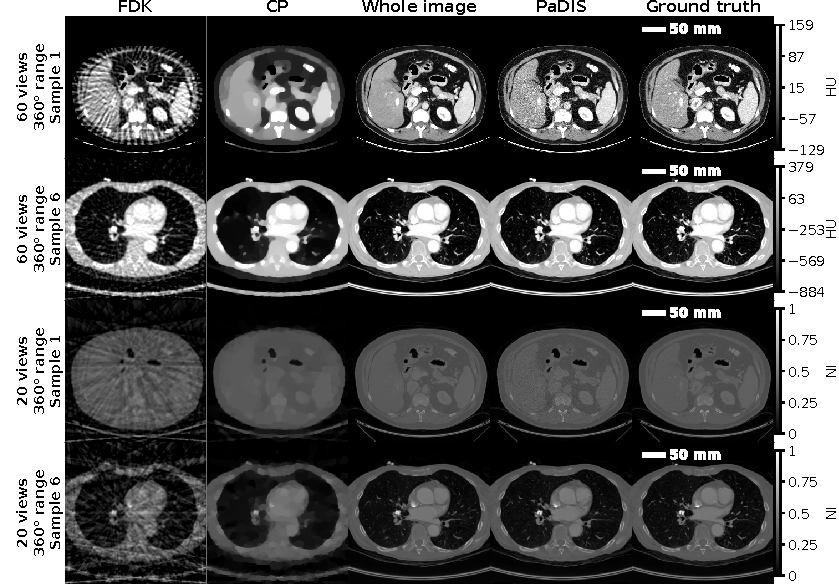
\includegraphics[width=0.90\textwidth]{Sections/4_results_figs/PDF/figure5_ct_reconstruction.pdf}
\caption{60-view HU (top) and 20-view NI (bottom) reconstructions comparing FDK, CP, whole-image VE-DPS and PaDIS-DPS.}
\label{fig:exec-ct}
\end{figure}

\section{Principal Findings}

The reconstructions in \autoref{fig:exec-ct} show representative fan-beam results from PaDIS and the comparison methods. On the exploratory four-image native $512\times512$ subset (\autoref{fig:exec-native}), LION-physics PaDIS achieved $40.08$ dB PSNR and $0.960$ SSIM, exceeding FDK and CP-TV without requiring a whole-image model at that resolution. The separately tuned PaDIS VE-DDNM configuration produced the best 20-view and 60-view PSNR values in this work, reaching $36.49$ and $41.55$ dB respectively, while the operator-normalised VE-DPS rows reduced relative sinogram residuals to approximately $10^{-3}$ and therefore kept the outputs closely tied to the measurements.

\begin{figure}[htbp]
\centering
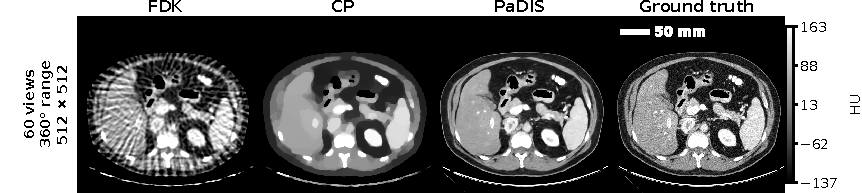
\includegraphics[width=0.90\textwidth]{Sections/4_results_figs/PDF/figure8_512_ct.pdf}
\caption{Native-resolution 60-view reconstruction, displayed in HU.}
\label{fig:exec-native}
\end{figure}

We did not reproduce the stronger claim of consistent PaDIS superiority. Under VE-DPS, the whole-image model achieved $34.25$ dB at 20 views and $29.58$ dB at 8 views, compared with $32.82$ and $27.65$ dB for PaDIS, and we observed the same reversal in the paper-style track. PaDIS exceeded the whole-image result only for some separately selected sampler configurations, notably VE-DDNM, so these comparisons do not isolate the prior alone. Patch training is therefore viable and sometimes advantageous, but the result depends on the interaction between prior, sampler and forward-operator scaling.

The ablations changed the interpretation further. A $96\times96$ patch model had almost the same mean PSNR as the whole-image model, while intermediate smaller patches performed worse, suggesting that global context remained valuable. However, the non-default patch and no-position models inherited the default PaDIS inference setting and were not individually optimised. Positional channels improved measurement-conditioned PSNR by only $0.3$ to $0.4$ dB, in contrast to the failure reported in the original PaDIS paper, and FDK and Gaussian initialisation converged to similar final quality. The geometric noise schedule instead improved PSNR by about $1.3$ dB over the released code's EDM-style default. Using all available training slices did not improve PaDIS under a fixed training-time budget, although fewer effective epochs mean this is not evidence that additional data are intrinsically unhelpful.

Among the four untuned samples per method in \autoref{fig:exec-generation}, random PaDIS partitions avoided the rectangular boundaries created by fixed patch stitching, although this small set cannot rank distributional quality. We recorded roughly two minutes per PaDIS slice, compared with about 2.6 minutes for whole-image VE-DPS and 24 minutes for fixed averaging or stitching, but concurrent jobs prevent an isolated speed comparison.

\section{Reproducibility, Limitations and Implications}

Exact reproduction of the original PaDIS paper was not possible. Important architecture information was distributed inconsistently between references, appendix and code \cite{}. Training patch counts, validation and checkpoint selection, test slice identities, complete physical geometry, and the hyperparameter search protocol were not specified. The original PaDIS paper and released code form a combined but internally inconsistent specification, containing materially different algorithmic choices \cite{}. By using three tracks, we made these differences explicit and showed that they can change scientific conclusions. The reversal of the central comparison is therefore an informative reproducibility result rather than a failed outcome.

This work remains limited to one dataset, simulated two-dimensional measurements and a small test set. Noise-free sinograms omit photon noise, scatter, beam hardening and motion, so we do not establish clinical low-dose performance. Some expensive experiments used only four images, confidence intervals do not include retraining variability, and no radiologist assessed lesion preservation or hallucination. A larger native-resolution test set is therefore needed before drawing a population-level comparison between reconstruction methods.

The practical conclusion is that PaDIS should be viewed as a memory-scalable route to high-resolution priors, not as a universally superior replacement for whole-image diffusion. Future work should use equal-compute and equal-epoch comparisons, multiple training seeds, calibrated measurement noise, external datasets and clinically relevant task assessment for safe clinical deployment. This work also demonstrates that inverse-problem papers should publish complete geometry, data splits, tuning procedures and code that matches the stated algorithms. Otherwise, apparent method improvements may instead reflect hidden implementation choices.

\begin{center}
\centering
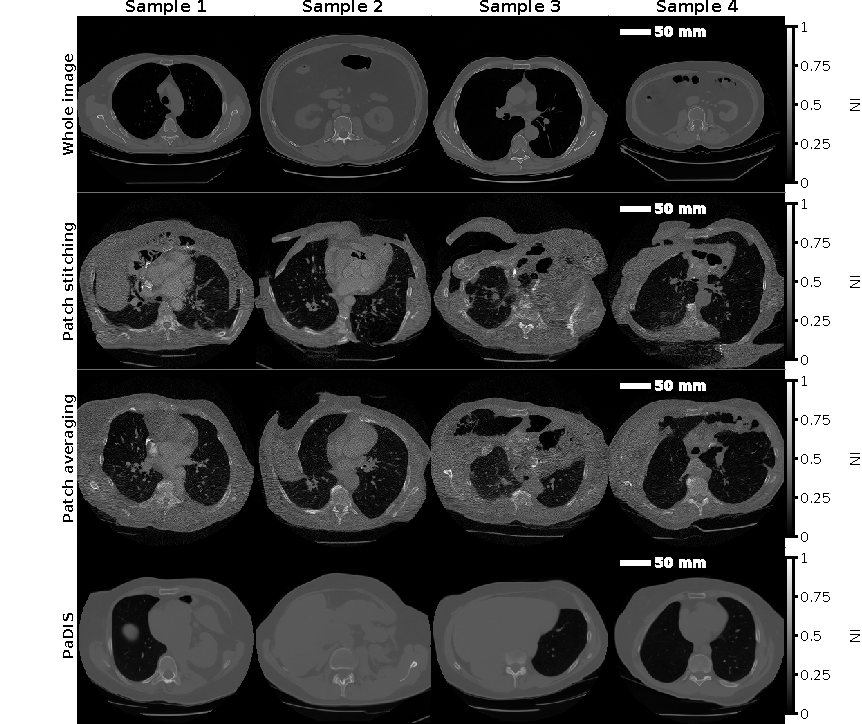
\includegraphics[width=0.64\textwidth]{Sections/4_results_figs/PDF/figure4_generation.pdf}
\captionsetup{type=figure}
\caption{Unconditional samples from whole-image, fixed patch-stitching, fixed patch-averaging and PaDIS priors, shown in NI.}
\label{fig:exec-generation}
\end{center}

\end{document}
